\documentclass[12pt,a4paper]{article}
\usepackage{graphicx}
\usepackage{wrapfig}
\usepackage{textcomp}
\usepackage{multicol}
\usepackage[utf8]{inputenc}

\title{Praktikum Physik - Dichte von Gasen}
\author{Simon Marti, Patricia Schwab, Mirco Kocher}
\date{11.05.2012}


\begin{document}
\maketitle

\section*{Ziel}
Bestimmung der Dichte f\"ur die Gase N$_2$, Ar und CO$_2$. Die Werte sollen danach mit den Literaturangaben verglichen werden.

\section*{Motivation}
Anhand dieses Experiments soll eine Methode zur Bestimmung der Dichte von drei allt\"aglichen Gasen erarbeitet werden.

\section*{Theorie}
Die gemessene Gewichtskraft $m^* \cdot g$ setzt sich aus folgenden Kr\"aften zusammen 
\begin{equation}
m^* \cdot g = Gas + Kolben - Waagschale - Auftrieb
\end{equation}
Das Gewicht des evakuierten Kolbens $m_0$ l\"asst sich mit dem Gewicht der Luft $m_{Luft}$, dem Restdruck $P_0$ und dem Luftdruck $P_L$ ermitteln
\begin{equation}
m_0 = m_{Luft} \frac{P_0}{P_L}
\end{equation}
\begin{equation}\label{eq:stp}
\rho_{STP} = \frac{\rho T P_{STP}}{P T_{STP}}
\end{equation}
Aus
\begin{eqnarray}
m^*_{Luft} & = & \rho _{Luft} V_I + m_{Kolben} - m_{Waagschale} - \rho_{Luft} V_A \label{eq:rl} \\
m^*_0 & = & \rho_{Luft} V_I \frac{P_0}{P_L} + m_{Kolben} - m_{Waagschale} - \rho_{Luft} V_A 
\end{eqnarray}
folgt
\begin{eqnarray}
m^*_0 - m^*_{Luft} & = & \rho_{Luft}V_I \left( \frac{P_0}{P_L}-1\right) \\
\Rightarrow \rho_{Luft} & = & \frac{m^*_0 - m^*_{Luft}}{V_I \left( \frac{P_0}{P_L}-1\right)} 
\end{eqnarray}
wobei $\rho_{Luft}$ die Dichte der Luft, $V_I$ das Innenvolumen und $V_A$ das Gesamtvolumen des Kolbens ist. \\
Durch Einsetzen von $\rho_{Luft}$ erh\"alt man
\begin{equation}\label{eq:const}
m_{Kolben} - m_{Waagschale} - \rho_{Luft} V_A = m^*_{Luft} - \rho _{Luft} V_I
\end{equation}
Nun kann die Dichte folgendermassen bestimmt werden
\begin{equation}\label{eq:rg}
\rho _{Gas} = \frac{m^*_{Gas} - (m_{Kolben} - m_{Waagschale} - \rho_{Luft} V_A)}{V_I}
\end{equation}


\section*{Aufbau und Ablauf}
\begin{multicols}{2}
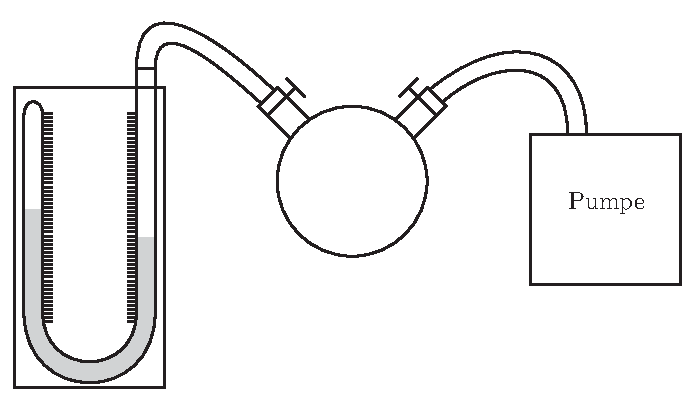
\includegraphics[width=6cm]{vakuum.pdf}

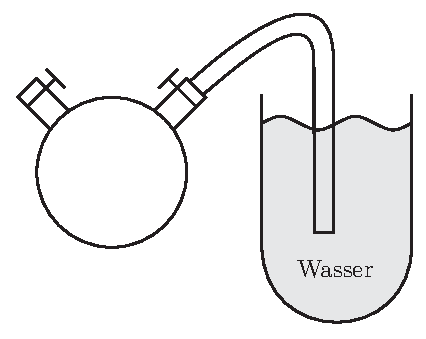
\includegraphics[width=5cm]{wasser.pdf}
\end{multicols}

\noindent
Ein Glaskolben ist mit Luft gefüllt und wird mit einer Balkenwaage gewogen um $m^*_{Luft}$ zu bestimmen. Als nächstes wird der Kolben mithilfe einer Vakuumpumpe evakuiert und erneut gewogen ($m^*_0$). Während dem evakuieren wird zudem der Restdruck $P_0$ mit einem Manometer gemessen. Nun wird der Kolben mit einem der drei Gasen gefüllt, erneut die Masse $m^*_{Gas}$ bestimmt und wieder evakuiert um das nächste Gas einfüllen zu können. Nachdem alle Gase gewogen wurden wird der Kolben mit Wasser gefüllt indem er erneut evakuiert und eines der Ventile in einem Wasserbecken geöffnet wird. Das Wasser im Kolben wird anschliessend in einem Messzylinder gemessen um $V_I$ zu bestimmen.

\section*{Rohdaten}
\begin{eqnarray*}
P_L & = & 721.7 \mbox{mmHg} \\
P_0 & = & 1 \mbox{Torr} \\
m^*_{Luft} & = & 146.77 \mbox{g} \\
m^*_{0} & = & 145.59 \mbox{g} \\
m^*_{CO_2} & = & 147.46 \mbox{g} \\
m^*_{Ar} & = & 147.28 \mbox{g} \\
m^*_{N_2} & = & 146.75\mbox{g} \\
\end{eqnarray*}


\section*{Auswertung}
Dichte der Luft nach (\ref{eq:rl})
\[ \rho_{Luft} = 1.1211 \mbox{kgm}^{-3} \]
Nach (\ref{eq:const})
\[ m_{Kolben} - m_{Waagschale} - \rho_{Luft} V_A = 0.1456 \mbox{kg} \]
Dichte der Gase nach (\ref{eq:rg})
\begin{eqnarray*}
\rho_{CO_2} = 1.776 \mbox{kgm}^{-3} \\
\rho_{Ar} = 1.605 \mbox{kgm}^{-3} \\
\rho_{N_2} = 1.102 \mbox{kgm}^{-3}
\end{eqnarray*}
Die Dichte konvertiert in STP nach (\ref{eq:stp})
\begin{eqnarray*}
\rho_{CO_2} = 2.038 \mbox{kgm}^{-3} \\
\rho_{Ar} = 1.842 \mbox{kgm}^{-3} \\
\rho_{N_2} = 1.265 \mbox{kgm}^{-3}
\end{eqnarray*}
\section*{Fehlerrechnung}


\section*{Diskussion}

\end{document}